\chapter{Results}
\label{sec:results}

This chapter will present the empirical results
of the branch-and-cut algorithm,
whose implementation was discussed in \cref{sec:implementation-chapter}.
We will evaluate its performance as a pricer for the CVRP,
by comparing it with
the state-of-the-art labeling algorithm based on dynamic programming
discussed in the works of \textcite{pessoa2020generic, sadykov2021bucket}.

\medskip

\section{CVRP Benchmark Instances}
\label{sec:results-benchmark-instances}

Several CVRP benchmark instances are mandated to measure the competitiveness
of our branch-an-cut pricer in an accurate manner.
The \urlref{http://vrp.galgos.inf.puc-rio.br/index.php/en/}{CVRPLIB website}
is an online database for the vehicle routing problem that includes
several downloadable test instances for free, among other things.
It is a valuable resource for all practitioners interested in the VRP.
It includes interactive plots of various routing problem instances
and the optimal (or best known) solution discovered by the best scholars over time.
Each CVRP test instance is stored in a file with the following filename template:
\begin{center}
	\begin{LVerbatim}
		<F>-n<N>-k<K>.vrp
	\end{LVerbatim}
\end{center}
where \texttt{.vrp} is the file extension,
\texttt{<N>} is the number of vertices in the instance, and
\texttt{<K>} is the number of (maximum or exact) available vehicles.
Finally, \texttt{<F>} represents the set instance family.
\texttt{<F>} is a single letter that uniquely identifies the instance
set and the authors who published such a set.
\texttt{P-n40-k5.vrp}, for example, denotes a test instance made up
of $40$ nodes ($39$ customers) and $5$ vehicles.
The \texttt{P} in the name refers to the instance set family,
which was published in \textcite{augerat1995}.

Each CVRP instance file's contents adhere
to the \texttt{TSPLIB95} file format \parencite{reinelt1995}.
Distances between pairs of nodes are computed
using the 2D Euclidean distance function rounded to the nearest integer,
as became standard for the TSP in \textcite{reinelt1991}.
Rounding is performed to stabilize the optimal values,
allowing for an accurate comparison of different contributions.
However, rounding introduces issues when comparing heuristic contributions;
for more information, see \textcite{uchoa2017}.

\medskip

We used some of the most historic and well-known CVRP instances to evaluate the performance of our pricer:
set A, B, P \parencite{augerat1995},
set E \parencite{dantzig1959, christofides1969, gaskell1967bases, gillett1974heuristic},
set F \parencite{fisher1994}
and finally set M \parencite{christofides1979vehicle}.
If the reader is wondering how these test sets were generated in the first place,
they can consult the CVRPLIB website or the work of \textcite{uchoa2017}.

The employed test instances are summarized in
\cref{table:cvrp-instance-family-E,table:cvrp-instance-family-F,table:cvrp-instance-family-A,table:cvrp-instance-family-B,table:cvrp-instance-family-P}.

\begin{table*}[thb]
	\centering
	% Place caption here to get a caption above the table
	\begin{tabular}[t]{lccc}
		\toprule
		\textbf{Instance} & $K$ & $Q$ & \textbf{Optimal Value} \\
		\midrule
		E-n51-k5          & 5   & 160 & 521                    \\
		E-n76-k7          & 7   & 220 & 682                    \\
		E-n76-k8          & 8   & 180 & 735                    \\
		E-n76-k10         & 10  & 140 & 830                    \\
		E-n76-k14         & 14  & 100 & 1021                   \\
		E-n101-k8         & 8   & 200 & 815                    \\
		E-n101-k14        & 14  & 112 & 1067                   \\
		\bottomrule
	\end{tabular}
	\caption{Instances of the set E employed for the empirical evaluation.
		These instances were originally proposed in \textcite{dantzig1959, christofides1969, gaskell1967bases, gillett1974heuristic}
		where the node locations were generated at random from a uniform distribution \parencite{uchoa2017}.
	}
	\label{table:cvrp-instance-family-E}
\end{table*}

\begin{table*}[thb]
	\centering
	% Place caption here to get a caption above the table
	\begin{tabular}[t]{lccc}
		\toprule
		\textbf{Instance} & $K$ & $Q$   & \textbf{Optimal Value} \\
		\midrule
		F-n45-k4          & 4   & 2010  & 724                    \\
		F-n72-k4          & 4   & 30000 & 237                    \\
		F-n135-k7         & 7   & 2210  & 1162                   \\
		\bottomrule
	\end{tabular}
	\caption{Instances of the set F employed for the empirical evaluation.
		These instances were originally proposed in \textcite{fisher1994},
		and they come from an actual distribution problem involving grocery deliveries in Ontario \parencite{uchoa2017}.
	}
	\label{table:cvrp-instance-family-F}
\end{table*}

\begin{table*}[thb]
	\centering
	% Place caption here to get a caption above the table
	\begin{tabular}[t]{lccc}
		\toprule
		\textbf{Instance} & $K$ & $Q$ & \textbf{Optimal Value} \\
		\midrule
		A-n37-k5          & 5   & 100 & 669                    \\
		A-n37-k6          & 6   & 100 & 949                    \\
		A-n38-k5          & 5   & 100 & 730                    \\
		A-n39-k5          & 5   & 100 & 822                    \\
		A-n39-k6          & 6   & 100 & 831                    \\
		A-n44-k6          & 6   & 100 & 937                    \\
		A-n45-k6          & 6   & 100 & 944                    \\
		A-n45-k7          & 7   & 100 & 1146                   \\
		A-n46-k7          & 7   & 100 & 914                    \\
		A-n48-k7          & 7   & 100 & 1073                   \\
		A-n53-k7          & 7   & 100 & 1010                   \\
		A-n54-k7          & 7   & 100 & 1167                   \\
		A-n55-k9          & 9   & 100 & 1073                   \\
		A-n60-k9          & 9   & 100 & 1354                   \\
		A-n61-k9          & 9   & 100 & 1034                   \\
		A-n62-k8          & 8   & 100 & 1288                   \\
		A-n63-k9          & 9   & 100 & 1616                   \\
		A-n64-k9          & 9   & 100 & 1401                   \\
		A-n65-k9          & 9   & 100 & 1174                   \\
		A-n69-k9          & 9   & 100 & 1159                   \\
		A-n80-k10         & 10  & 100 & 1763                   \\
		\bottomrule
	\end{tabular}
	\caption{Instances of the set A employed for the empirical evaluation.
		These instances were originally proposed in \textcite{augerat1995}
		where the node locations are generated at random on a square grid \parencite{uchoa2017}.
	}
	\label{table:cvrp-instance-family-A}
\end{table*}

\begin{table*}[thb]
	\centering
	% Place caption here to get a caption above the table
	\begin{tabular}[t]{lccc}
		\toprule
		\textbf{Instance} & $K$ & $Q$ & \textbf{Optimal Value} \\
		\midrule
		B-n38-k6          & 6   & 100 & 805                    \\
		B-n39-k5          & 5   & 100 & 549                    \\
		B-n41-k6          & 6   & 100 & 829                    \\
		B-n43-k6          & 6   & 100 & 742                    \\
		B-n44-k7          & 7   & 100 & 909                    \\
		B-n45-k6          & 6   & 100 & 678                    \\
		B-n50-k7          & 7   & 100 & 741                    \\
		B-n50-k8          & 8   & 100 & 1312                   \\
		B-n51-k7          & 7   & 100 & 1032                   \\
		B-n52-k7          & 7   & 100 & 747                    \\
		B-n56-k7          & 7   & 100 & 707                    \\
		B-n57-k7          & 7   & 100 & 1153                   \\
		B-n57-k9          & 9   & 100 & 1598                   \\
		B-n63-k10         & 10  & 100 & 1496                   \\
		B-n64-k9          & 9   & 100 & 861                    \\
		B-n66-k9          & 9   & 100 & 1316                   \\
		B-n67-k10         & 10  & 100 & 1032                   \\
		B-n68-k9          & 9   & 100 & 1272                   \\
		B-n78-k10         & 10  & 100 & 1221                   \\
		\bottomrule
	\end{tabular}
	\caption{Instances of the set B employed for the empirical evaluation.
		These instances were originally proposed in \textcite{augerat1995}
		where the node locations are generated at random on a square grid \parencite{uchoa2017}.
	}
	\label{table:cvrp-instance-family-B}
\end{table*}

\begin{table*}[thb]
	\centering
	% Place caption here to get a caption above the table
	\begin{tabular}[t]{lccc}
		\toprule
		\textbf{Instance} & $K$ & $Q$  & \textbf{Optimal Value} \\
		\midrule
		P-n16-k8          & 8   & 35   & 450                    \\
		P-n19-k2          & 2   & 160  & 212                    \\
		P-n20-k2          & 2   & 160  & 216                    \\
		P-n21-k2          & 2   & 160  & 211                    \\
		P-n22-k2          & 2   & 160  & 216                    \\
		P-n22-k8          & 8   & 3000 & 603                    \\
		P-n23-k8          & 8   & 40   & 529                    \\
		P-n40-k5          & 5   & 140  & 458                    \\
		P-n45-k5          & 5   & 150  & 510                    \\
		P-n50-k7          & 7   & 150  & 554                    \\
		P-n50-k8          & 8   & 120  & 631                    \\
		P-n50-k10         & 10  & 100  & 696                    \\
		P-n51-k10         & 10  & 80   & 741                    \\
		P-n55-k7          & 7   & 170  & 568                    \\
		P-n55-k8          & 8   & 160  & 588                    \\
		P-n55-k10         & 10  & 115  & 694                    \\
		P-n55-k15         & 15  & 70   & 989                    \\
		P-n60-k10         & 10  & 120  & 744                    \\
		P-n60-k15         & 15  & 80   & 968                    \\
		P-n65-k10         & 10  & 130  & 792                    \\
		P-n70-k10         & 10  & 135  & 827                    \\
		P-n76-k4          & 4   & 350  & 593                    \\
		P-n76-k5          & 5   & 280  & 627                    \\
		P-n101-k4         & 4   & 400  & 681                    \\
		\bottomrule
	\end{tabular}
	\caption{Instances of the set P employed for the empirical evaluation.
		These instances were originally proposed in \textcite{augerat1995}
		obtained from modifying the capacities of some instances of the A, B and E sets \parencite{uchoa2017}.
	}
	\label{table:cvrp-instance-family-P}
\end{table*}


\subsection{Inflation of the CVRP Test Instances}
\label{sec:inflation-of-the-cvrp-test-instances}

We created new artificial instances based on the presented sets in
\cref{table:cvrp-instance-family-E,table:cvrp-instance-family-F,table:cvrp-instance-family-A,table:cvrp-instance-family-B,table:cvrp-instance-family-P}.
The idea is to generate new CVRP instances characterized by longer routes
so that we can evaluate the behavior of the proposed branch-and-cut pricer and labeling algorithm
as the routes they need to produce grow longer (see previous discussions in
\cref{sec:intro-thesis-contributions,sec:solving-the-pricing-problem}).
The new artificial instances were created as follows.
Let $Q \in R_+,\ k \in Z_+$ respectively denote the vehicle
capacity and the number of trucks of the unmodified CVRP instance.
Define a scale factor $s \in R_+$.
For each unmodified CVRP instance, we generate a new artificial instance
characterized by the vehicle capacity $Q^\prime \in R_+$
and by the number of vehicles $k^\prime \in Z_+$.
We've inflated the total number of available CVRP instances
by using the following relationship:
$$
	Q^\prime = Q \times s, \quad K^\prime = \ceil*{\frac{K}{s}}
$$
Inflation is performed for each unmodified CVRP instance by using
multiple values for the scale factor $s \in R_+$.
As $s \in R_+$ grows, the inflated CVRP instances will look more and more like a conventional TSP.
If $\ceil*{\frac{K}{s}} = 1$ the CVRP decades to a TSP and, as a result,
the BAP frameworks may become a suboptimal approach for dealing with such a problem.

\section{\bapcod{}}
\label{sec:results-bapcod}

\bapcod{} \parencite{sadykov2021} is a software package
developed in France at the Bordeaux University and Bordeaux Research Center
that embeds a sophisticated column generation approach
embedded in a generic and modern branch-price-and-cut (BPC) algorithm.
\bapcod{} takes a compact mixed-integer programming model as input
and solves it using a Dantzig-Wolfe reformulation \parencite{dantzig1960}.
See the previous discussion on \cref{sec:set-partitioning-formulation,sec:branch-and-price}.
The modern BPC solver automatically applies the Dantzig-Wolfe reformulation.
In this case, a default generic pricer based on a MIP optimizer
is employed during the column generation phase.
\bapcod{} uses an automatic dual price smoothing stabilization,
as discussed in \textcite{pessoa2018automation},
to improve the convergence speed of the column generation.
\bapcod{} supports direct branching on the master formulation's arc-flow variables
as well as Vanderbeck branching \parencite{vanderbeck2011}.
The latter is a non-robust branching scheme imposing bounds modifications on the sub-problem variables.
Because \bapcod{} is generic, it supports user-developed extensions
which can alter the BPC algorithm's behaviour.
These extensions can provide the BPC framework with
custom-defined cutting planes (robust and non-robust),
custom branching decisions (robust and non-robust),
or even ad-hoc pricer implementations.

The \vrpsolver{} extension \parencite{pessoa2020generic}, is
a \bapcod{} extension distributed by the same authors.
This extension includes an
advanced implementation of a bidirectional dynamic programming labeling algorithm
\parencite{sadykov2021bucket} for solving the pricing problem.
The included labeling algorithm
can be used as an exact or heuristic pricer.
The labeling algorithm contains two successively lighter heuristic implementations;
for more information, see \textcite{sadykov2021bucket}.
The labeling algorithm makes use of a generalized ng-sets definition \parencite{baldacci2011}
defined through the \textit{packing} and \textit{elementarity} sets,
as described in \textcite{pessoa2020generic}.
When the solution obtained after the CG convergence is fractional,
the ng-sets are dynamically augmented,
see \textcite{pessoa2020generic} for more details.
The \vrpsolver{} extension, also,
includes the implementation of some
specific cutting planes and branching decisions
aimed at efficiently solving routing-like problems
(or problems that exhibit similar structures)
such as the CVRP, VRPTW, and also others (see \cite{pessoa2020generic}).
The \vrpsolver{} implements the robust RCC cuts of \textcite{laporte1983},
and the non-robust limited-memory rank-1 cuts of \textcite{pecin2017improved}.
The \vrpsolver{} also implements the non-robust Ryan\&Foster branching \parencite{ryan1981integer}.
The \vrpsolver{} extension was also used successfully in \textcite{pessoa2020}
to solve the Bin Packing Problem (BPP).

\medskip

Currently, \bapcod{} and its \vrpsolver{} extension are the leading cutting-edge technologies
for solving vehicle routing problems \parencite{pessoa2020generic}.
The \bapcod{} source code is available for free, for academic purposes only,
by issuing a form request to this URL: \url{https://bapcod.math.u-bordeaux.fr/}.
The \vrpsolver{} extension, on the other hand, is only available in compiled form,
and must be explicitly requested via email by contacting one of the
original authors: \url{mailto:ruslan.sadykov@inria.fr}.
The official technical report presented in \textcite{sadykov2021} contains instructions
for building, configuring, and using \bapcod{} and its \vrpsolver{} extension.
To round things out, a Julia language interface to the \vrpsolver{} extension
can be found at this \urlref{https://github.com/inria-UFF/BaPCodVRPSolver.jl}{Github repo}.

For a comprehensive technical discussion of the components of
modern and advanced BPC frameworks, see \textcite{sadykov2019modern}.

\section{Evaluation Setup}
\label{sec:results-evaluation-setup}

The goal of this thesis, as previously stated,
is to determine whether a branch-and-cut framework can be competitive in solving the pricing problem,
particularly as the produced routes grow in length.
We hypothesized that, since the labeling algorithm's performance degrades
as the vehicle capacity increases,
a branch-and-cut framework could aid in solving the more demanding pricing problems.
Refer back to the discussion in \cref{sec:intro-thesis-contributions,sec:solving-the-pricing-problem}
for additional details.

However, the two frameworks operate in very different ways.
Our branch-and-cut framework does not support non-robust inequalities or variable fixing
but produces stronger dual bounds.
Similarly, the labeling algorithm instead generates weaker dual bounds
but allows for multiple column generation per pricing invocation,
non-robust cut generations and branching.
As a result, comparing the performance of the two schemes is not an easy task.
So a natural question arises.
What is the best approach to compare the performance of the two frameworks?

\medskip

When it came to developing our branch-and-cut pricer, we had two options:
(i) developing our pricer in tight integration with the BPC framework, by coding it as a \bapcod{} plugin,
or (ii) developing the pricer in a standalone executable, separate from the BPC framework.

The first option has two primary benefits.
For starters, it enables our branch-and-cut pricer to influence the BPC algorithm's execution flow.
Second, it empowers more diversified ways of measuring the pricer's effectiveness.
We can decide to compare
the running time required for solving the root node, the running time for solving the entire CVRP instance
or the running time of each single pricing iteration.
The disadvantage of the first approach is its implementation complexity
and constraint in tooling or programming languages employed.
Programming the BAC pricer as \bapcod{} plugin requires heavy knowledge of this BPC algorithm's intricacies.

The second option, on the other hand, has one significant advantage:
it allows for greater implementation flexibility, simplifying development efforts.
We can develop the BAC pricer in complete isolation,
using whatever programming language or external library we want.
However, the branch-and-cut pricer cannot change the BPC algorithm's execution flow.
As a result, the branch-and-cut pricer follows the same execution flow
as the BPC algorithm  using the labeling algorithm.
This scenario led to two primary downsides.
For starters, improved dual-bounds from the BAC algorithm
will not affect the number of pricing iterations.
As a result, the BAC algorithm's solution to the more difficult elementary SPPRC
has no practical way to pay off its high computation times.
Secondly, the time required to solve each pricing iteration
is the only viable metric to measure the pricers' competitiveness.

\medskip

In the end, we decided on the second option.
We chose simplicity over complexity and built our pricer as a standalone executable.
Measuring the running time of each pricing iteration is neither an appropriate nor a poor approach.
There are both benefits and downsides to this approach.
First \bapcod{} must be configured to operate in the same domain as our pricer,
thereby disabling many features that could potentially result in high efficiency in the broader scheme.
Second, our branch-and-cut pricer generates elementary bounds, naturally solving a harsher problem.
While solving a single pricing iteration may take longer,
stronger dual-bounds may skip some pricing iterations in the long run,
thus resulting in an overall faster CVRP resolution.
On the other hand, measuring the pricers' efficiency per each single pricing iteration,
it is straightforward to assess compared to the alternative approaches described.

Summing up, it is clear that the performance comparison that we've settled on is just
a mere indicator of the genuine efficiency of the two approaches and must
therefore be taken cautiously.
We believe, however, there is still value in performing such a comparison as it provides
a first proof-of-concept/direction regarding the feasibility of the effectiveness
of a branch-and-cut scheme for addressing the pricing problem.

\medskip

We conclude this section by introducing the \bapcod{} parametrization,
which we used to bend the labeling algorithm to operate in a compatible environment for the BAC algorithm.

The configuration parameters are specified separately
in an appropriately placed configuration file.
The BPC framework's branching and cut-generation schemes have been disabled,
thus asking the algorithm to halt at the root node of the branch-and-bound tree.
We enabled the ng-sets' augmentation and set the maximum ng-set threshold as high as possible,
therefore putting pressure on the labeling algorithm to generate dual bounds as close
to the elementary bound as possible at the end of each CG iteration.
The pricer's tailing-off condition was disabled.
We've also asked the labeling algorithm to generate
a single column per pricing invocation.
Refer to \cref{sec:bapcod-appendix} for a complete list of the employed configuration.

\section{Evaluation Process}
\label{sec:results-evaluation-process}

We employed \bapcod{} version 0.66 (released in November 2021) and the \texttt{libRCSP v0.5.12}.
The latter library contains the \vrpsolver{} extension's implementation.
The goal is to use \bapcod{} to solve many CVRP instances while simultaneously
measuring the labeling algorithm's running at each pricing invocation.

\medskip

We re-adapted one of the VRPTW examples (included in the distribution)
to model a Capacitated Vehicle Routing Problem by following
the \bapcod{} technical document of \textcite{sadykov2021}.
The master formulation that we've implemented follows the two-index arc flow model
presented in \cref{eq:two-index-flow-obj-func,eq:two-index-flow-two-edges-incident-per-customer,eq:two-index-flow-two-k-edges-incident-in-the-depot-node,eq:two-index-flow-ccc,eq:two-index-flow-x-mip-var-bounds-depot,eq:two-index-flow-x-mip-var-bounds},
excluding the Rounded Capacity Constraints (RCC) of \cref{eq:two-index-flow-ccc}.

To use the \vrpsolver{} extension's labeling algorithm,
the associated Resource Constrained Shortest Path (RCSP) sub-problem must be defined.
The RCSP sub-problem is formulated on a complete directed network by
linking the new RCSP modeling variables to the master problem formulation.
The RCSP sub-problem necessitates the correct definition of the following:
the source/sink vertices, as well as the so-called \textit{packing} and \textit{elementarity} sets
(see \cite{pessoa2020generic} for more details).
The correct definition of these generalized sets is required
for specific components  of the \vrpsolver{} extension to function properly (ng-sets, RCC separation, etc).
For each customer, a unique \textit{packing} set and \textit{elementarity} set are created.
The \vrpsolver{} extension also necessitates the explicit definition of an additional
distance matrix encoding the distance between pairs of elementarity sets.
The elementarity sets and the distance matrix specified by the user
let \bapcod{} compute the ng-sets automatically.

Due to internal implementation details of \bapcod{},
the RCSP sub-problem requires the user to specify the consumptions (or demand) for each network's arc.
Resource consumptions cannot aren't definable at the vertex level.
Therefore, as suggested in \textcite{pessoa2020generic}, we have defined the resource consumption
on the arcs as $q_{ij} = \frac{q_{i} + q_{j}}{2} \quad \forall i, j \in V$.
This definition is valid and it leads to a symmetric resource consumption ($q_{ij} = q_{ji}$).
The symmetric resource consumption property improves the efficiency in pricing
by eliminating the need for backward labeling \parencite{pessoa2020generic}.

We implemented a custom pricing functor to extract the information
required for the performance evaluation.
The pricing functor is essentially a glorified callback
that can be used to solve the pricing problem through user-defined custom code.
Our pricing functor is a simple stubbed implementation
that ultimately invokes the pricing functor of  the standard \vrpsolver{} extension.
However, before calling the labeling algorithm, we first do the following.
First, we assess the labeling algorithm's performance by measuring its running time.
Second, at each pricing invocation, we record the dual variables $\pi \in \R^N$ of the RMP
to be later dumped into a dedicated file.

Because of the implementation details of \bapcod{},
the reduced cost of an edge does not follow the simple relationship
$\bar{c}_{ij} = c_{ij} - \frac{\pi_i + \pi_j}{2} \quad \forall i, j \in V,\ i \ne j$.
By accessing an appropriate field on the MP formulation structure,
the user can retrieve the dual variables $\pi_0 \in R$.
The remaining dual variables $\pi_i \quad \forall i \in V_0$
must be calculated from the reduced cost of each edge $\bar{c}_{ij}$.
Internally, \bapcod{} encodes the reduced cost of an edge using the following relationship:
\begin{equation}
	\bar{c}_{ij} = \begin{cases}
		c_{ij} - \frac{\pi_{j}}{2}       & \texttt{if } i = 0, j \in V_0       \\
		c_{ij} - \frac{\pi_i + \pi_j}{2} & \texttt{if } i, j \in V_0,\ i \ne j
	\end{cases}
	\label{eq:bapcod-encoded-reduced-cost-vars}
\end{equation}
By exploiting \cref{eq:bapcod-encoded-reduced-cost-vars},
we've implemented a trivial recursive algorithm
to extract all the necessary dual variables $\pi \in \R^N$.

In conclusion, we save two files to the hard drive for each pricing invocation of the labeling algorithm.
The first file is a JSON file that contains metadata information about
the labeling algorithm, such as the instance name, the instance size,
the total running time for the labeling, the reduced cost of the generated route
and the column generation iteration.
The second file, instead, encodes a CPTP instance including:
the dual variables (the vertices' profit),
the original demands, the original node positions, and the vehicle capacity.
The CPTP instance is encoded in a slightly modified TSPLIB95 file format.
In the file format, we've added a new dedicated section, called \texttt{PROFIT\_SECTION},
to hold the extracted dual variables.

\subsection{Performance profiles}
\label{sec:results-performance-profiles}

\textit{Performance profiles}, first introduced in \textcite{dolan2002},
are a plot representation used to benchmark optimization software.
These novel plot representations are easy to interpret and less susceptible to personal interpretation.
In a nutshell, performance profiles represent the cumulative distribution function of a performance metric.
We put $H$ algorithms to the test by running them through $M$ problem instances.
The metric under consideration in \textit{performance profiles}
is typically the overall running time of an algorithm.
When the metric under measurement is the running time, we obtain the so-called \textit{time profiles}.

In \textit{time profiles}, the time ratio relative to a baseline is plotted on the X-axis.
The baseline is calculated as the best performance obtained from all the algorithms under consideration.
Instead, the Y-axis depicts the likelihood of being within an X ratio of the baseline.
In \textit{time profiles}, the ideal solver appears as a straight vertical line on the entire left of the plot.
An example of a \textit{time profile} is provided in \cref{fig:example-of-time-profile-tsp}.

In our case, we also employ the so-called \textit{cost profiles} to plot either the optimal value
or the best dual-bound found from each algorithm.
Instead of computing its ratio w.r.t. a baseline, the raw value of the metric is plotted directly.
Recording the dual bounds inside a \textit{cost profile}
allows us to select the best algorithm
based on its convergence speed over a limited time frame (time-limit).
When plotting the optimal value in the \textit{cost profiles}, on the other hand,
we can validate the pricer that would feed the BPC framework with tighter dual bounds.
Because the optimal value $z$ always satisfies $z \le 0$,
we used two sentinel values to accentuate some specific circumstances.
When a pricer successfully determines that no reduced cost route exists
($z \ge \varepsilon_{\mt{ct}}$,
we output $z = 1.0$ in the associated performance profile.
Instead, if the pricer fails to solve the PP optimally within the timelimit,
we output $z = 2.0$.

\medskip

In this thesis, we evaluated the efficiency of our proposed BAC-based pricer
using both the \textit{cost and time profiles}.
Our pricer's efficiency is compared to the RCSP dynamic programming algorithm
included in the \vrpsolver{} extension \parencite{pessoa2020generic} of \bapcod{}.

\begin{figure}[t]
	\centering
	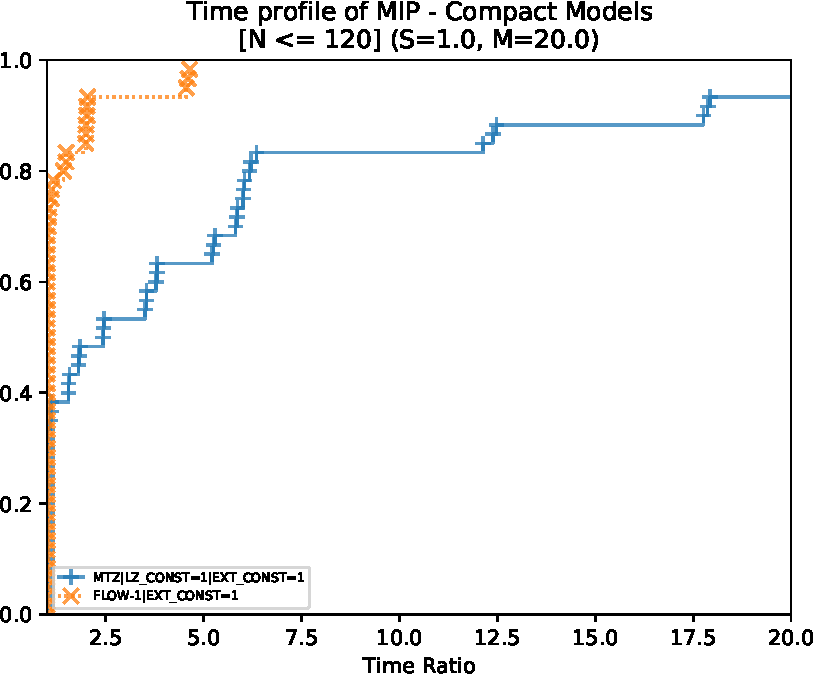
\includegraphics[width=\textwidth]{./Imgs/perfprof-tsp-example/time-ratio20.0.cropped.pdf}
	\caption{
		This example of a \textit{time profile} depicts two exact algorithms for the TSP under analysis.
		A vertical straight line on the entire left side of the plot would represent the best scenario.
		In the situation depicted in the figure, the algorithm named \texttt{FLOW-1|EXT\_CONST=1} outperforms the other algorithm in the vast majority of cases.
	}
	\label{fig:example-of-time-profile-tsp}
\end{figure}

\section{Empirical Results}
\label{sec:results-empirical-results}

\mytodo{Describe that only the last 10 pricing instances were used for comparison}

\mytodo{Describe operating system, processor speed, etc}

\mytodo{Introduce common issues in performance evaluation of chaotic systems. Solution through randomized runs with different starting seeds}

\mytodo{Report timelimit, seed values. num threads of the MIP optimizer}

\mytodo{Spam this section with performance profiles}

% TODO(dparo): First batch: 1 Thread, 60 seconds of timelimit, we compare the dual bounds

% TODO(dparo): second batch: 16 threads, 20 minutes of timelimit


\newcommand{\IncludePerfProfSubFiguresBatchOne}[1]{
	\begin{subfigure}{0.30\textwidth}
		\centering
		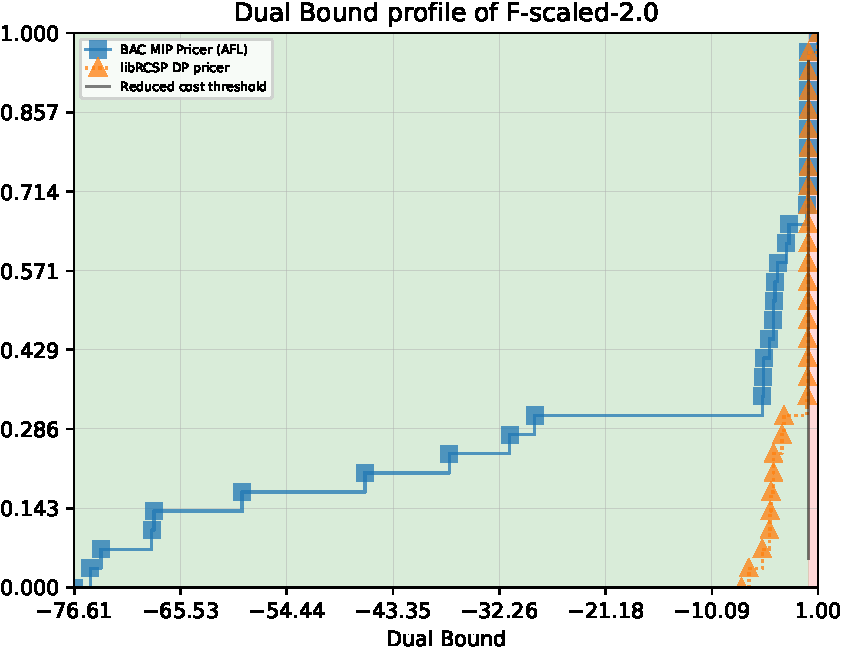
\includegraphics[width=1.0\linewidth]{./Imgs/perfprofs/#1/DualBound_plot.cropped.pdf}
	\end{subfigure}
}

\begin{figure}[t]
	\IncludePerfProfSubFiguresBatchOne{Fractional-labeling-comparison-for-E-scaled-1.0}
	\hfill
	\IncludePerfProfSubFiguresBatchOne{Fractional-labeling-comparison-for-E-scaled-2.0}
	\hfill
	\IncludePerfProfSubFiguresBatchOne{Fractional-labeling-comparison-for-E-scaled-4.0}

	\IncludePerfProfSubFiguresBatchOne{Fractional-labeling-comparison-for-F-scaled-1.0}
	\hfill
	\IncludePerfProfSubFiguresBatchOne{Fractional-labeling-comparison-for-F-scaled-2.0}
	\hfill
	\IncludePerfProfSubFiguresBatchOne{Fractional-labeling-comparison-for-F-scaled-4.0}

	\IncludePerfProfSubFiguresBatchOne{Fractional-labeling-comparison-for-A-scaled-1.0}
	\hfill
	\IncludePerfProfSubFiguresBatchOne{Fractional-labeling-comparison-for-A-scaled-2.0}
	\hfill
	\IncludePerfProfSubFiguresBatchOne{Fractional-labeling-comparison-for-A-scaled-4.0}

	\IncludePerfProfSubFiguresBatchOne{Fractional-labeling-comparison-for-B-scaled-1.0}
	\hfill
	\IncludePerfProfSubFiguresBatchOne{Fractional-labeling-comparison-for-B-scaled-2.0}
	\hfill
	\IncludePerfProfSubFiguresBatchOne{Fractional-labeling-comparison-for-B-scaled-4.0}

	\IncludePerfProfSubFiguresBatchOne{Fractional-labeling-comparison-for-P-scaled-1.0}
	\hfill
	\IncludePerfProfSubFiguresBatchOne{Fractional-labeling-comparison-for-P-scaled-2.0}
	\hfill
	\IncludePerfProfSubFiguresBatchOne{Fractional-labeling-comparison-for-P-scaled-2.0}

	\caption{
		This empirical study investigates the tightness of the dual bound for various versions of the BAC algorithm.
		The plots are laid out in a matrix format.
		Each row corresponds to a unique CVRP test set.
		From top to bottom: \texttt{E}, \texttt{F}, \texttt{A}, \texttt{B} and finally \texttt{P}.
		Each column represents a different inflation scale factor $s$.
		From left to right: $s = 1$, $s = 2$ and finally $s = 4$.
		The version that uses amortized fractional labeling (\texttt{AFL}), represented here by the orange line, appears to produce tighter dual bounds in the majority of cases.
	}
	\label{fig:perfprofs-batch1-part1}
\end{figure}

\newcommand{\IncludePerfProfSubFigures}[1]{
	\begin{subfigure}{0.45\textwidth}
		\centering
		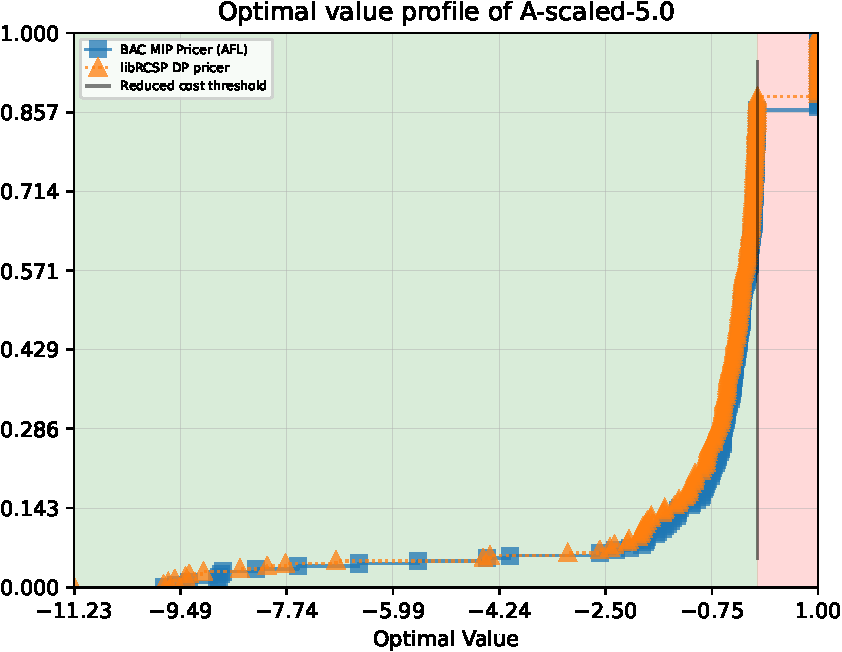
\includegraphics[width=1.0\linewidth]{./Imgs/perfprofs/#1/OptimalValue_plot.cropped.pdf}
	\end{subfigure}
	\hfill
	\begin{subfigure}{0.45\textwidth}
		\centering
		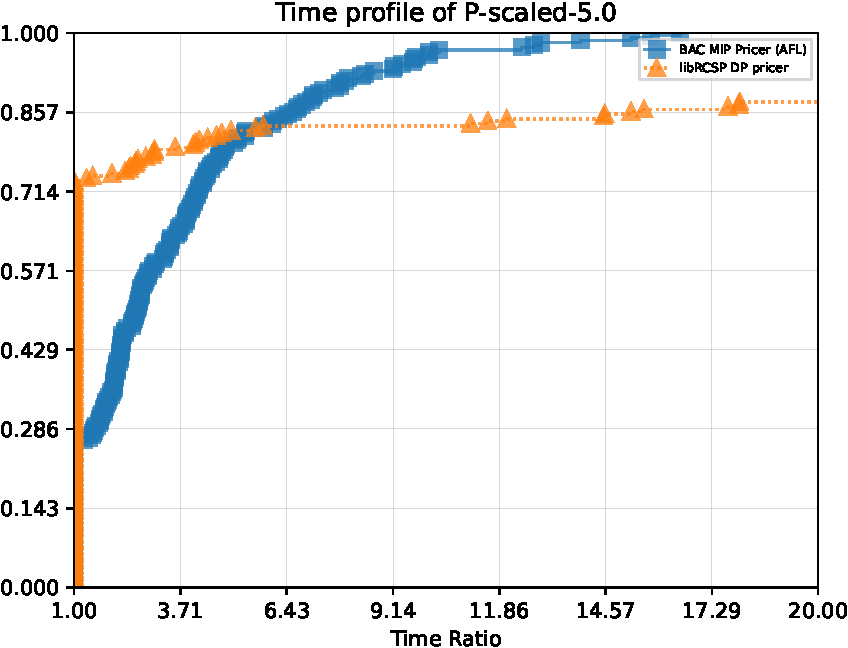
\includegraphics[width=1.0\linewidth]{./Imgs/perfprofs/#1/Time_plot.cropped.pdf}
	\end{subfigure}%
}

\newcommand{\PerfprofFigureCaptionOne}[1]{
	Empirical study comparing the pricing performance of the proposed BAC-pricer to the labeling algorithm of \textcite{pessoa2020generic} on the \texttt{#1} test set.
	On the left, the cost profile representing the optimal value found by each method.
	On the right, the time profile measuring the time ratio of the two approaches.
	Each row represents a different inflation scale factor $s$.
	From top to bottom: $s = 1, 2 \text{ and } 4$.
}

\newcommand{\PerfprofFigureCaptionTwo}[1]{
	Continuation of the empirical study of \cref{fig:perpfrofs-batch2-#1-part1} testing even further inflation scale factors: $s = 5, 8, 10 \text{ and } 20$.
}

\newcommand{\PerfprofFiguresPartOne}[1]{
	\begin{figure}[t]
		\IncludePerfProfSubFigures{#1-scaled-1.0}
		\vspace{2.5mm}

		\IncludePerfProfSubFigures{#1-scaled-2.0}
		\vspace{2.5mm}

		\IncludePerfProfSubFigures{#1-scaled-4.0}

		\caption{\PerfprofFigureCaptionOne{#1}}
		\label{fig:perpfrofs-batch2-#1-part1}
	\end{figure}
}

\newcommand{\PerfprofFiguresPartTwo}[1]{
	\begin{figure}[t]
		\IncludePerfProfSubFigures{#1-scaled-5.0}
		\vspace{2.5mm}

		\IncludePerfProfSubFigures{#1-scaled-8.0}
		\vspace{2.5mm}

		\IncludePerfProfSubFigures{#1-scaled-10.0}
		\vspace{2.5mm}

		\IncludePerfProfSubFigures{#1-scaled-20.0}

		\caption{\PerfprofFigureCaptionTwo{#1}}
		\label{fig:perpfrofs-batch2-#1-part2}
	\end{figure}
}

\newcommand{\PerfprofFigures}[1]{
	\PerfprofFiguresPartOne{#1}

	\PerfprofFiguresPartTwo{#1}

}

\forcsvlist{\PerfprofFigures}{E,F,A,B,P}


\begin{comment}
Each performance profile follows the syntax:
\begin{center}
	\begin{LVerbatim}
		<FAMILY-NAME>-scaled-<s>-last-10
	\end{LVerbatim}
\end{center}
where \texttt{<FAMILY>} denotes the CVRP instances family (i.e. E, F, etc) and \texttt{<s>} is the scale factor for the vehicle capacity.
The term \texttt{last-10} is used to denote that the performance profile uses only the last 10 pricing iterations for performing the comparison.

At the time of writing, only the following scaling factors were tested: $s = 1.0,\ s = 2.0,\ s = 4.0$.
\end{comment}

\begin{comment}
[@dparo: Old Gomoru HU Tree, It was slow and required amortization to speed up the BAC procedure]
In this implementation we employed the usage of both the push relabel algorithm,
the Gomory-Hu tree and full enumeration of all possible $(s, t)$ vertices.
Since running this full enumeration over each fractional separation,
turned out to be quite costly, we decided to amortize the cost over multiple iterations.
Namely, fractional separations iterations which are not multiple of $N$ become a no-op,
no maxflow is performed and therefore no set $S \subseteq V_0$ is separated.
\end{comment}

\section{Discussion of the Empirical Results}
\label{sec:results-discussion}

\mytodo{Discuss the performance profiles here}

\begin{comment}
\begin{landscape}
	\begin{table}[ht]
		\centering
		\begin{tabular}{l|lll|lll|lll|lll|}
			\multirow{3}{*}{Original CVRP Instance} & \multicolumn{6}{c|}{scaled 1.0} & \multicolumn{6}{c|}{scaled 2.0}                                                                                                                \\
			\cmidrule{2-7}
			                                        & \multicolumn{3}{c|}{libRCSP}    & \multicolumn{3}{c|}{BAC MIP}    & \multicolumn{3}{c|}{libRCSP} & \multicolumn{3}{c|}{BAC MIP}                                                  \\
			                                        & UB                              & LB                              & T [s]                        & UB                           & LB & T [s] & UB & LB & T [s] & UB & LB & T [s] \\
			\toprule
			A-n37                                   & x0                              & y0                              & t0                           & x1                           & y1 & t1    & x0 & y0 & t0    & x1 & y1 & t1    \\
			A-n38                                   & x2                              & y2                              & t2                           & x3                           & y3 & t3    & x2 & y2 & t2    & x3 & y3 & t3    \\
			\bottomrule
		\end{tabular}
	\end{table}
\end{landscape}

\end{comment}

\begin{comment}
\mytodo{Include the F-n135 grep result to talk about the difficulty of this instance and related ones}
\end{comment}
